
\begin{exercise}
Show that the Edmonds-Karp algorithm terminates after $n \cdot m$ iterations of the 
while-loop. \textbf{Hint.} Initially, compute an optimal $k$-layering (which?). Then keep
this layering as long as its optimal. Once it ceases to be optimal, compute a new optimal
layering. Note that the Edmonds-Karp algorithm does not actually need to compute any
layering. It's us who compute it to show that $n \cdot m$ bound on the number of iterations.
\end{exercise}

\begin{proof}
First we construct an optimal layering by breath first search. We have to make sure that the $t \in V_k$, so whenever BFS reaches $t$, we should put $t$ and the rest of vertices to $V_k$ and stop BFS. 
\par According to $ex.10.8$, after at most $m$ iterations of Edmonds-Karp algorithm, the optimal $k$-layering ceases to be optimal, which means $dist_G\left(s,t\right)>k$. Then we will do BFS again to create a $k'$-layering, where $k'=dist_G\left(s,t\right)>k$. The maximum times we can add $k$ by one is the number of vertices, that means we go through $0$ layering to $n-1$ layering. So the algorithm terminates after $n\cdot m$ iterations.

%Then there exist $V_i$ such that $x,y \in V_i$, $x,y$ are two neighoring vertices on the shortest path from $s$ to $t$, as the picture shows.
%\begin{center}
%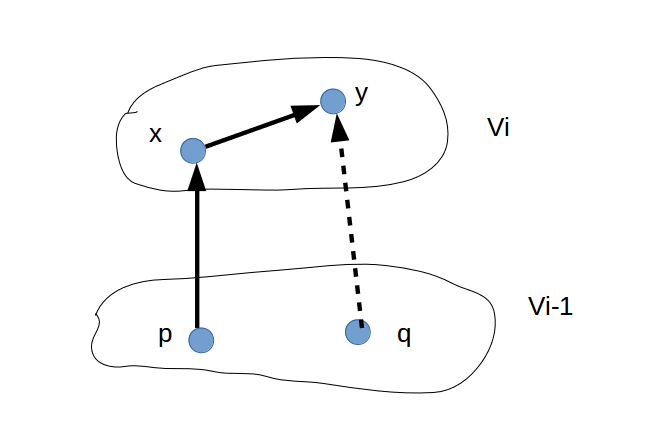
\includegraphics[width=0.6\textwidth]{figures/Ex10-9.png}
%\end{center}
\end{proof}

\begin{exercise}
   Show that every network has a maximum flow $f$. 
   That is, a flow $f$ such that ${\rm val}(f) \geq {\rm val}(f')$ for every flow $f'$.
   \textbf{Remark.} This sounds obvious but it is not. In fact, there might be an infinite
   sequence of flows $f_1, f_2, f_3, \dots$ of increasing value that does not reach any maximum.
    Use the previous exercises!
\end{exercise}

\begin{proof}
According to ex10.9, we know that the Edmonds-Karp algorithm terminates after $n \cdot m$ iterations of the while-loop. At each iteration, the increase of flow is a finite value because capacity of edges is finite. The final flow is the sum of limited number of finite value, so it is reachable.  
\end{proof}

